% !TEX encoding = UTF-8
% !TEX TS-program = pdflatex
% !TEX root = ../Tesi.tex
% !TEX spellcheck = en-EN

%************************************************
\chapter{Artificial Neural Network}
\label{cap:ann}
%************************************************

\section{Probability theory}
\label{sec:probability}

\citet{RefWorks:194} defines $X$ a random variable with a fixed domain $Val(X)$,
showing aspects of the system's world. In this world, a fixed assignment of
values to variables (from one to all) is called an $event$.
Given a probability distribution $P$, this assigns to the specific event
$\alpha$ a value: $P(\alpha)$.
Provided a random variable $X$, whose $Val(X) = \{ x^1, \ldots , x^k \}$, a
\textit{Probability Distribution} over $X$ is $P(X) = \{ P(x^1), \ldots , P(x^k)
\}$.
He further defines, given a second random variable $Y$:
\begin{itemize}
  \item {Probability of conjunction of events, $P(X = x, Y = y)$ or $P(x, y)$,
  or $P((X = x) \cap (Y = y))$;}
  \item {A set of variables, $\mathbf{X} = \{X_1, X_2, \ldots , X_k \}$;}
  \item {Joint distribution over one set of variables, $P(\mathbf{X}) =
  P(X_1, X_2, \ldots , X_k) $;}
  \item {Joint distribution over two sets of variables, $P(\mathbf{X, Y}) =
  P(X_1, X_2, \ldots , X_k, Y_1, Y_2, \ldots , Y_l  ) $;}
  \item {Conditional distribution, $P(\mathbf{X | Y}) =
  P(X_1, X_2, \ldots , X_k | Y_1, Y_2, \ldots , Y_l  ) $.}
\end{itemize}

For later reference, we write two fundamental rules of the probability theory,
the sum rule (Eq. \ref{eq:sumrule}) and the product rule (Eq.
\ref{eq:productrule}), from which Bayes derived his theorem (Eq.
\ref{eq:bayestheorem}):
\begin{equation}
\label{eq:sumrule}
P(X) = \sum_Y {P(X, Y)}, 
\end{equation}

\begin{equation}
\label{eq:productrule}
P(X, Y) = P(Y | X) \cdot P(X), 
\end{equation}

\begin{equation}
\label{eq:bayestheorem}
P(Y | X) = \frac{P(X | Y) \cdot P(Y)}{P(X)}.
\end{equation}


\subsection{The Gaussian Distribution}
\label{subsec:gaussian}

Provided a single real valued variable $x$, a Gaussian distribution is:
\begin{equation}
\label{eq:gaussiandistribution}
\mathcal{N}(x | \mu, \sigma^2) = \frac{1}{(2 \pi \sigma^2)^{0.5}} exp \left\{
 - \frac{1}{2 \sigma^2} (x - \mu)^2	\right\} ,
\end{equation}

where $\mu$ is the mean and $\sigma^2$ is the variance, of which the square root
is the standard deviation.
Further, $\beta = 1/\sigma^2$ is the deviation.
Given a set of observations $\mathbf{x} = (x_1, \ldots, x_N)^T$, assumed
\textit{indipendent and identically distributed} (i.i.d.), the probability of
the data set becomes:
\begin{equation}
\label{eq:likelihoodgaussian}
p(\mathbf{x} | \mu, \sigma^2) = \prod_{n = 1}^{N} \mathcal{N}(x | \mu,
\sigma^2),
\end{equation}
which can be more easily computed if written in a logaritmic form:
\begin{equation}
\label{eq:loglikelihoodgaussian}
ln p(\mathbf{x} | \mu, \sigma^2) = - \frac{1}{2 \sigma^2} \sum_{n = 1}^{N}{(x_n
- \mu)^2} - \frac{N}{2} ln (\sigma^2) - \frac{N}{2} ln (2 \pi) .
\end{equation}
To obtain the expectation of this likelihood Equation
\ref{eq:loglikelihoodgaussian} can be maximized over $\mu$ and $\sigma^2$,
giving respectively Eq. \ref{eq:mu} and Eq. \ref{eq:sigma}:
\begin{equation}
\label{eq:mu}
\mathbb{E}[\mu_{ML}] = \mathbb{E}\left[\frac{1}{N} \sum_{n =
1}^{N}{(x_n)}\right] = \mu ,
\end{equation}
\begin{equation}
\label{eq:sigma}
\mathbb{E}[\sigma^2_{ML}] = \mathbb{E}\left[\frac{1}{N} \sum_{n = 1}^{N}{(x_n -
\mu_{ML})^2} \right] = \left( \frac{N - 1}{N} \right) \sigma^2.
\end{equation}
In case of a D-dimensional vector $\mathbf{x}$, we write the multivariate
Gaussian distribution as:
\begin{equation}
\label{eq:multivariategaussiandistribution}
\mathcal{N}(\mathbf{x} | \boldsymbol{\mu}, \mathbf{\Sigma}) = 
\frac{1}{(2 \pi)^{D/2} |\boldsymbol\Sigma|^{0.5}} 
exp \left\{ - \frac{1}{2} (\mathbf{x} - \boldsymbol{\mu})^T 
\boldsymbol\Sigma^{-1}  (\mathbf{x} - \boldsymbol{\mu})
\right\} ,
\end{equation}

where $\mathbf{\Sigma}$ is the covariance matrix.


\section{Regression statistics}
\label{sec:regressionstatistics}

Statistics finds relationship between random variables.
Once one of them ($response$) is chosen, it infers its dependance from the
others ($regressors$), also including an additive $error$ term
(\citet{RefWorks:194}). We call this a \textit{regression model}, which can be
linear or nonlinear.
In this work we exploited the following regression models:
\begin{itemize}
  \item{Bayesian linear,}
  \item{Gaussian non linear,}
  \item{Artificial Neural Network (\acs{ANN}).}
\end{itemize}
We later explained, section \ref{sec:annmodeldev}, why we focused on the last
one over the other two.
% The B and the  regressions 
% can be used as regression methods for \acs{DEM} identification
% and as benchmark for more precise tools. 
%to further
%assess the quality of the \acs{ANNs} training.

\subsection{Supervised learning}
\label{subsec:supervisedlearning}

The learning processes available for a regression model are:

\begin{itemize}
  \item{supervised learning, or learning with a teacher,}
  \item{semi-supervised learning,}
  \item{unsupervised learning.}
\end{itemize}

The easiest regression model consists in fitting target data
points (exptected response) with a polynomial curve.
The cofficients of the curve are obtained by minimizing a cost function, which
is proportional to the distance of said data points to the curve.
The expected response represents the teacher of the system.
The network is trained in \textit{batch mode}, all the examples are known before
starting the training.
Further, these examples were assumed to be \textit{independent and identically
distributed}.
We focused on supervised learning: the materials we investigated
are examined in batch, not online.\\
\citet{RefWorks:194} defines \textit{supervised learning} an application, where all the
training examples comprises the input vectors and their corresponding target
vectors.
%\subsection{Gaussian non linear regression}
%\label{subsec:gaussiannonlinearregression}
% \improvement{I focus only on supervised learning, but also unsupervised
% learning and semi-supervised learning exist.}


\subsection{The Standard Bayesian Linear Model}
\label{subsec:standardlinearmodel}

\citet{RefWorks:192} define the standard linear regression model with Gaussian noise as:
\begin{equation}
\label{eq:standardlinearregression}
y = \mathbf{x}^T \mathbf{w} + \varepsilon,
\end{equation}

where $\mathbf{x}$ is the input vector, $\mathbf{w}$ are the weights of the
linear model, and $y$ is the target value. The noise $\varepsilon$ adopts an
$i.i.d.$ Gaussian distribution:
\begin{equation}
\label{eq:noise}
\varepsilon = \mathcal{N}(0, \sigma_n^2).
\end{equation}

Extending to the n-dimensional case, we have a set of $n$ observations:
\begin{equation}
\label{eq:observations.tex}
\mathcal{D} = \{ (\mathbf{x}_i, y_i) | i = 1, \ldots, n \} = (X, \mathbf{y}).
\end{equation}

Consequently, the $likelihood$, or probability density of the observations given
the parameters, becomes:
\begin{equation}
\label{eq:likelihoodcontinuous}
\begin{align*}
p(\mathbf{y} | X, \mathbf{w}) &= \prod_{i = 1}^{n} {p(y_i | \mathbf{x}_i,
\mathbf{w})} = \prod_{i = 1}^{n} {\frac{1}{\sqrt{2\pi} \sigma_n} 
exp \left(- \frac{(y_i - \mathbf{x}_i^T \mathbf{w})^2}{2 \sigma_n^2} \right)} \\
&= \frac{1}{(2\pi \sigma_n^2)^{n/2}} exp \left(- \frac{1}{2 \sigma_n^2}
|\mathbf{y} - X^T \mathbf{w}|^2 \right) = \mathcal{N}(X^T \mathbf{w}, \sigma_n^2
I), 
\end{align*}
\end{equation}
where the Euclidean length of vector $\mathbf{v}$ is indicated by
$|\mathbf{v}|$.
We also consider the weights $\mathbf{w}$ proportional to the Gaussian
distribution with zero mean and variance equal to the coviarance matrix
$\Sigma_p$.\\
Remembering the theorem of Bayes, Eq. \ref{eq:bayestheorem}, which states that:
\begin{equation}
\label{eq:bayestheoremword}
posterior = \frac{likelihood \times prior}{marginal ~ likelihood},
\end{equation}

we can define the continuous posterior distribution as:
\begin{equation}
\label{eq:bayestheoremcontinuous}
p(\mathbf{w | y }, X) = \frac{p(\mathbf{y} | X, \mathbf{w}) \cdot
p(\mathbf{w})}{p(\mathbf{y} | X)},
\end{equation}

where the \textit{marginal likelihood} is:
\begin{equation}
\label{eq:marginallikelihood}
p(\mathbf{y} | X) = \int{p(\mathbf{y} | X, \mathbf{w} p(\mathbf{w}) d
\mathbf{w}}.
\end{equation}

A first estimation of the posterior can be determined as follow:
\begin{equation}
\label{eq:likelihoodprior}
\begin{align*}
p(\mathbf{w} | X, \mathbf{y}) 
& \propto exp(- \frac{1}{2 \sigma_n^2} (\mathbf{y} - X^T \mathbf{w})^T
(\mathbf{y} - X^T \mathbf{w})) exp(- \frac{1}{2} \mathbf{w}^T \Sigma_p^{-1}
\mathbf{w}) \\
& \propto exp(- \frac{1}{2} (\mathbf{w} - \mathbf{\bar{w}})^T (\frac{1}{
\sigma_n^2} X X^T + \Sigma_p^{-1}) (\mathbf{w} - \mathbf{\bar{w}}))  \\
& \sim \mathcal{N}( \mathbf{\bar{w}} = \frac{1}{\sigma_n^2} A^{-1} X
\mathbf{y}, A^{-1}) ,
\end{align*}
\end{equation}

where $A = \sigma_n^{-2} X X^T + \Sigma_p^{-1}$.\\
An effective tool for the posterior predictive density of a variational Bayesian
multiple linear regression model is provided by \citet{RefWorks:193}.
% % \subsection{Bayesian linear regression}
% \label{subsec:bayesianlinearregression}

% We chose the Bayesian inference amongst the possible linear regression models.
%     a_0: shape parameter of the prior precision of coefficients
%     b_0: rate  parameter of the prior precision of coefficients
%     c_0: shape parameter of the prior noise precision
%     d_0: rate  parameter of the prior noise precision

% The theory is briefly explained in subsection \ref{subsec:bayesian linear
% regression}.
% \wrong{understand if the software requires as priors only the standard
% deviation or also the initial weights.}
% \info{to be continued}

\subsection{Gaussian Process}
\label{subsec:gaussianprocess}

\citet{RefWorks:192} define a \textit{Gaussian process} as a set of random variables. 
Any finite random of these variables have a joint Gaussian distribution.
The process $f(\mathbf{x})$ can be defined by its mean function $m(\mathbf{x})$
and its covariance function $k(\mathbf{x, x'})$, which are, respectively:
\begin{equation}
\label{eq:meanfunction}
m(\mathbf{x}) = \mathbb{E}\left[f(\mathbf{x}) \right],
\end{equation}
\begin{equation}
\label{eq:covariancefunction}
k(\mathbf{x, x'}) = \mathbb{E}\left[(f(\mathbf{x}) - m(\mathbf{x}))
(f(\mathbf{x'}) - m(\mathbf{x'})) \right],
\end{equation}
and it can be written in a compact form as:
\begin{equation}
\label{eq:gaussianprocess}
f(\mathbf{x}) \sim \mathcal{GP}(m(\mathbf{x}), k(\mathbf{x, x'})).
\end{equation}
In fact, the Bayesian linear regression model is a subcase of the Gaussian
process model, with the following conditions:
\begin{equation}
\label{eq:bayesianlinearmodelgaussianprocess}
\begin{align*}
f(\mathbf{x}) &= \boldsymbol{\phi(\mathbf{x})}^T \mathbf{w}, \\
\mathbf{w}	  & \sim \mathcal{N} (\mathbf{0}, \Sigma_p), \\
\mathbb{E}[f(\mathbf{x}) ] &= \boldsymbol{\phi(\mathbf{x})}^T
\mathbb{E}[\mathbf{w}] = 0, \\
\mathbb{E}[f(\mathbf{x}) f(\mathbf{x'})] &= \boldsymbol{\phi(\mathbf{x})}^T
\mathbb{E}[\mathbf{ww}^T] \boldsymbol{\phi(\mathbf{x'})} =
\boldsymbol{\phi(\mathbf{x})}^T \Sigma_p \boldsymbol{\phi(\mathbf{x'})}.
\end{align*}
\end{equation}
We used the \textit{squared exponential} (SE), also called Radial Basis Function
(RBF) or Gaussian Function, as covariance function. It defines the covariance
between a pair of random variables as:
\begin{equation}
\label{eq:covariancefunctionse}
cov(f(\mathbf{x}_p), f(\mathbf{x}_q)) = k(\mathbf{x}_p, \mathbf{x}_q) =
exp \left(-\frac{1}{2} |\mathbf{x}_p - \mathbf{x}_q|^2 \right) .
\end{equation}

Specifically, we handled the software developed by \citet{RefWorks:192} 
for Gaussian processes inference and prediction, although we constrained ourselves to the case of exact inference
(regression with Gaussian likelihood).
The complete description of the Gaussian non linear regression can be found in
\citet{RefWorks:194}.

\info{decide if using the equations from 5.3 to 5.7 of Rasmussen}

\section{Introduction on Artificial Neural Networks}
\label{sec:annintro}
%\improvement{Add some more details from Haykin introduction}
An Artificial Neural Network (\acs{ANN}) is a powerful regression model, 
based on non-linear functions (\citet{RefWorks:158}). 
In fact, we can see a neural network as a huge and parallel computer, composed
of many processing units. 
It stores experienced knowledge and translates it in
an usable form. 
The biological inspiration for artificial neural networks can be seen in Fig.
\ref{fig:049neuron1}. 
It resembles the human brain especially because it
uses a learning process to acquire knowledge, which is stored through the
synaptic weights.

\begin{figure}[!htb]
\centering
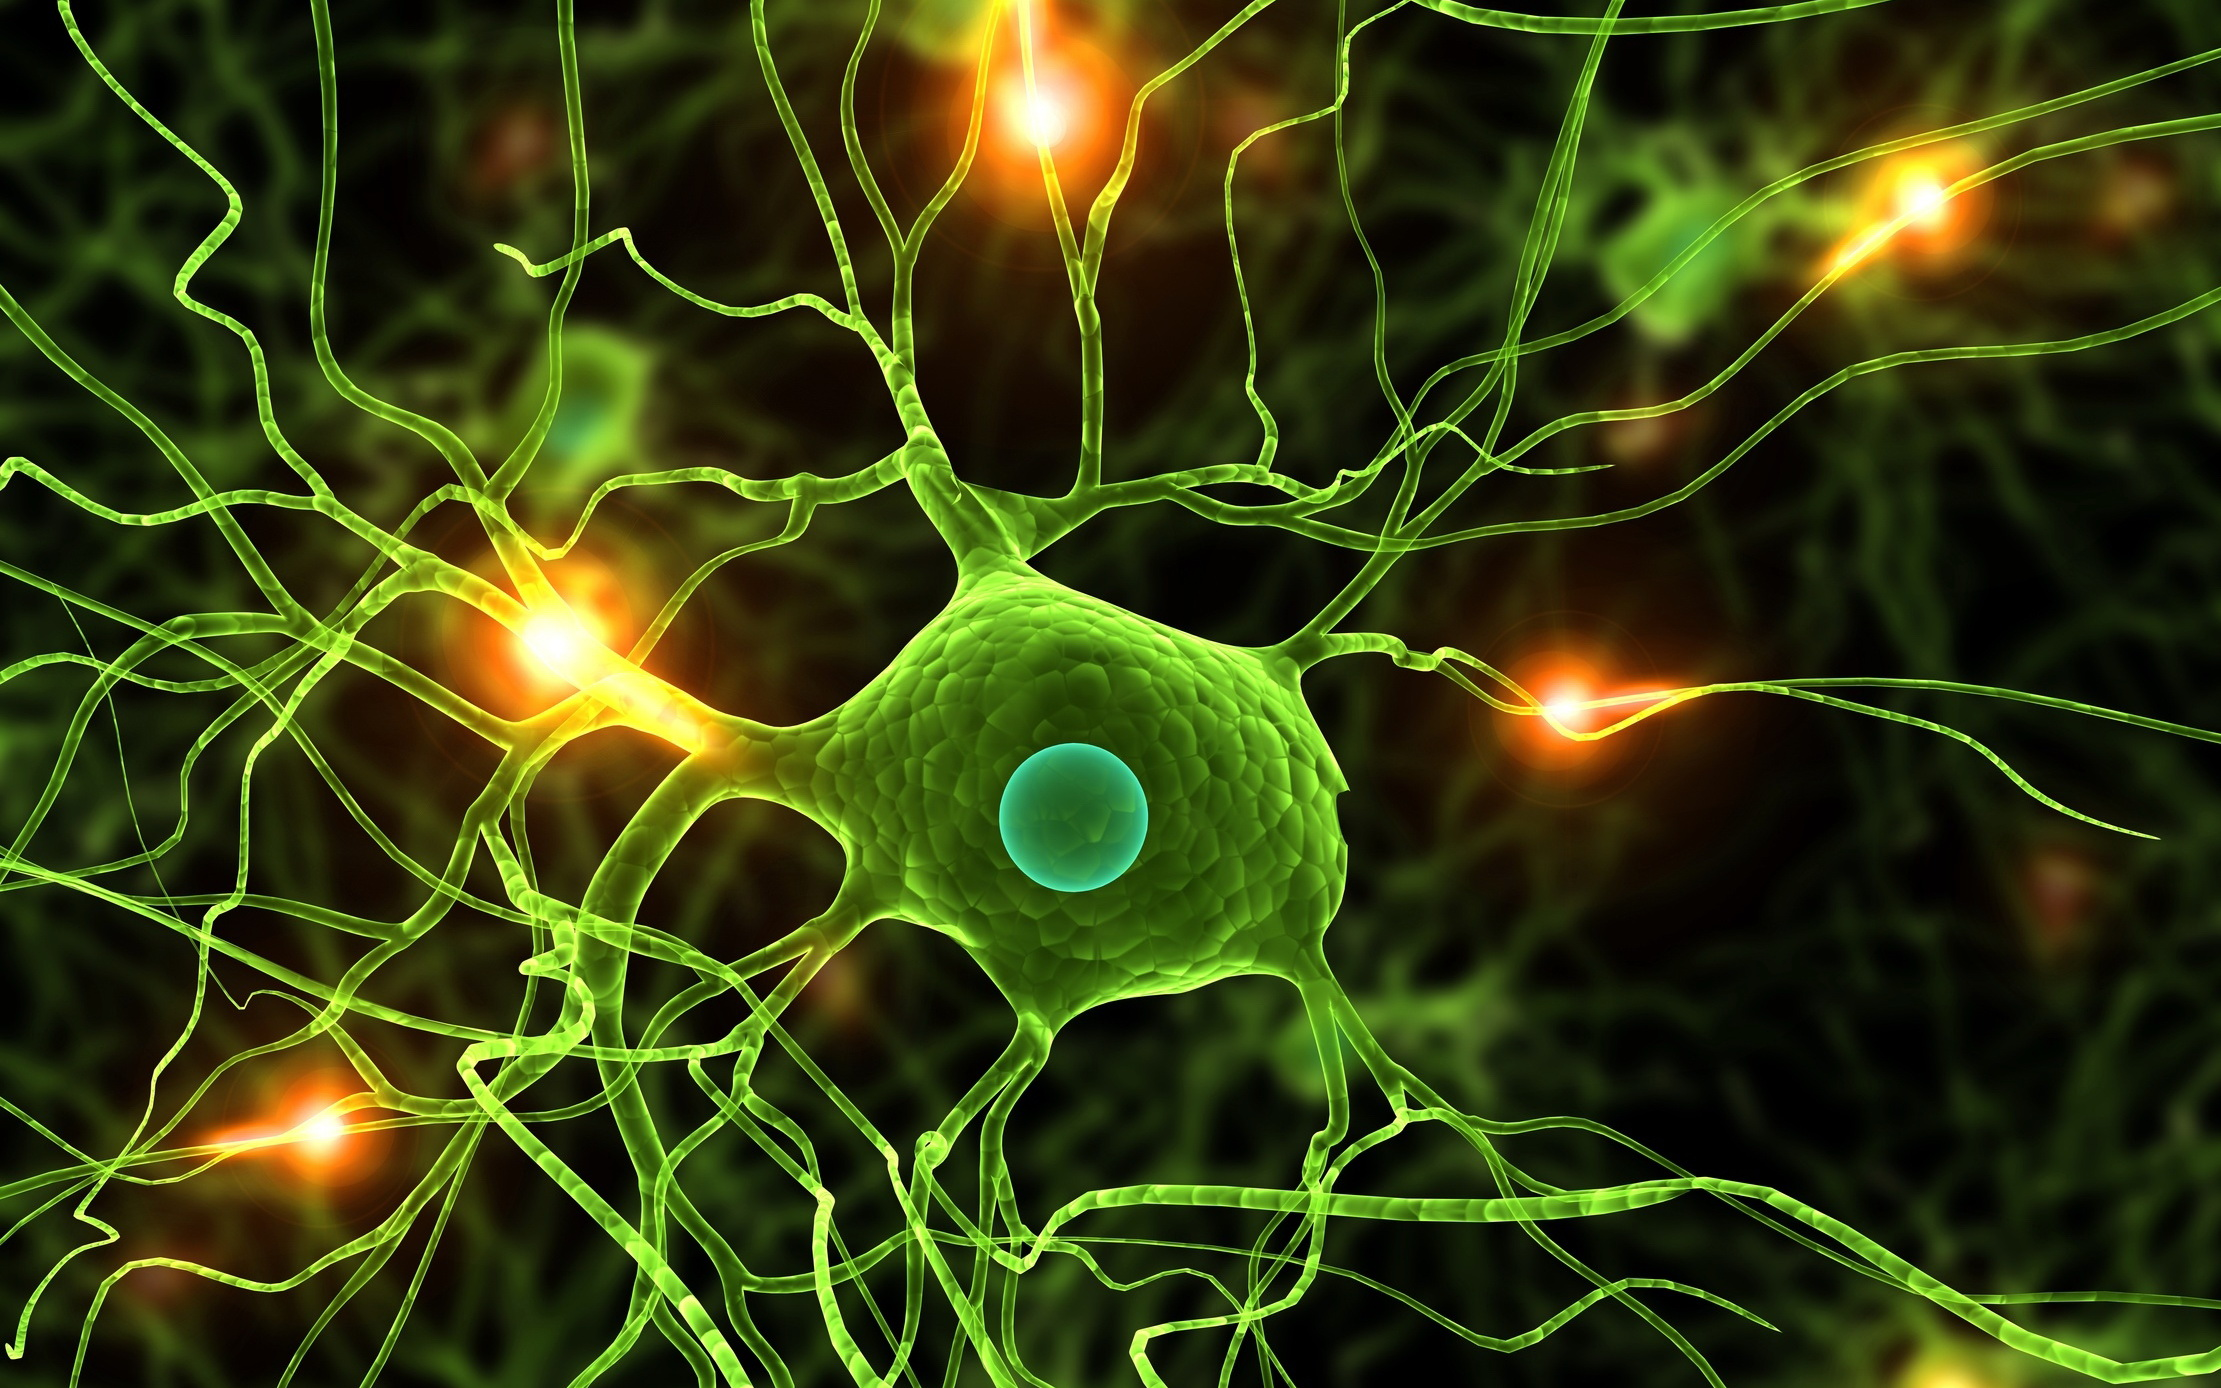
\includegraphics[width=.80\columnwidth]{images/049neuron1}
\caption[Biological inspiration 2]{Biological inspiration 2.}
\label{fig:049neuron1}
\end{figure}

In this work, we first used the \acs{ANN} to fit the \acs{DEM} numerical simulation
data, and then to process a vast number of parameters combinations. 
\acs{ANNs} map combinations of input data to convenient outputs (fitting). 
Amongst the available \acs{ANNs} were important for our context: 
\begin{itemize}
  \item {the Feedforward (\acs{FF}) \acs{ANN},}
  \item {the Radial basis function (\acs{RBF}) \acs{ANN}.}	
\end{itemize}
We did not investigate the latter.
For \acs{FF}-\acs{ANN},
numerous training algorithms are available. 
The most common are based on
backpropagation, e.g., Levenberg-Marquardt, Bayesian regulation and the scaled
conjugate gradient.

\section{Perceptron}
\label{sec:perceptron}

The basic element of an artificial neural network is the perceptron, a single
neuron, see Fig.
\ref{fig:064perceptron}
It is composed by inputs ($x_1, x_2, \ldots, x_m$), weights for these inputs
($w_1, w_2, \ldots, w_m$) and a bias $b$.
A linear combination of these elements, and the incorporation of the bias, 
forms the induced local field \cite{RefWorks:158}: 
\begin{equation}
v = b + \sum_{j = 1}^{m}{w_j \cdot x_j},
 \label{eq:inducedlocalfield}
\end{equation}

or hard limiter.
Then, we can obtain the output $y$ thanks to the activation function
$\varphi(\cdot)$:
\begin{equation}
y = \varphi(b + \sum_{j = 1}^{m}{w_j \cdot x_j}),
 \label{eq:perceptron}
\end{equation}

\begin{figure}[!htb]
\centering
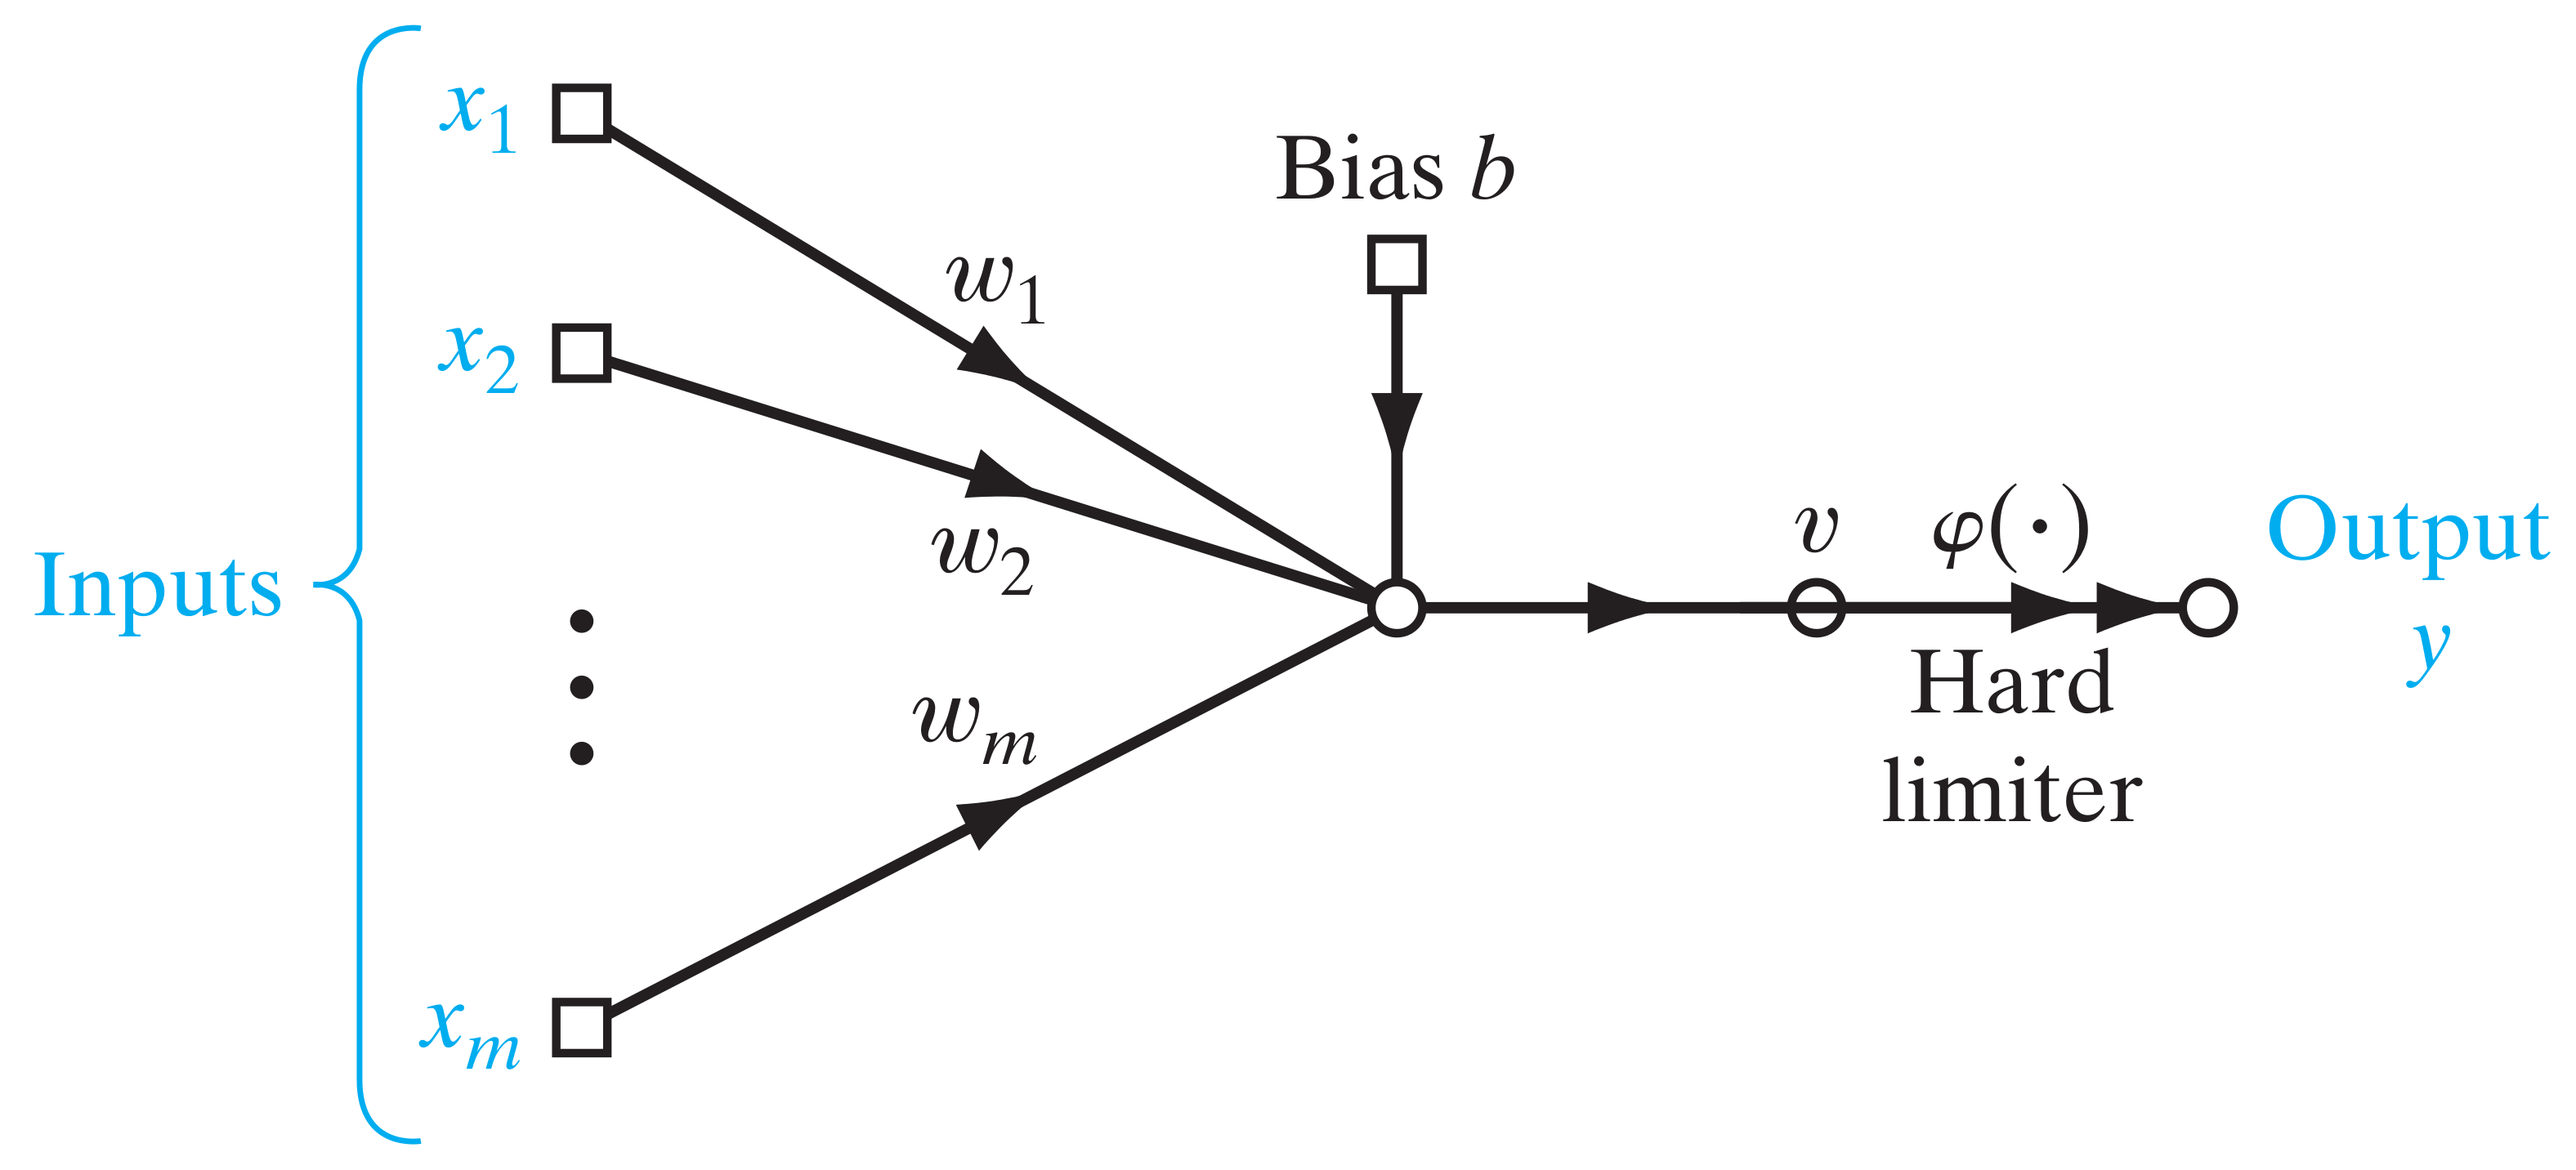
\includegraphics[width=.80\columnwidth]{images/064perceptron}
\caption[Perceptron scheme]{Perceptron scheme \cite{RefWorks:158}.}
\label{fig:064perceptron}
\end{figure}
In the simplest case the activation function $\varphi(\cdot)$ is a signum function.
Consequently, $y$ can be +1, for positive inputs, or -1, for negative inputs. Inputs of the first class
belong to class $\mathscr{C}_1$, of the second to class $\mathscr{C}_2$.
Thus, the patterns ($y$) are hypothesised to be linearly separable.
In this case the training, as identification of the correct weights and bias,
can be precisely mathematically described. \\
\begin{figure}[!h]
\centering
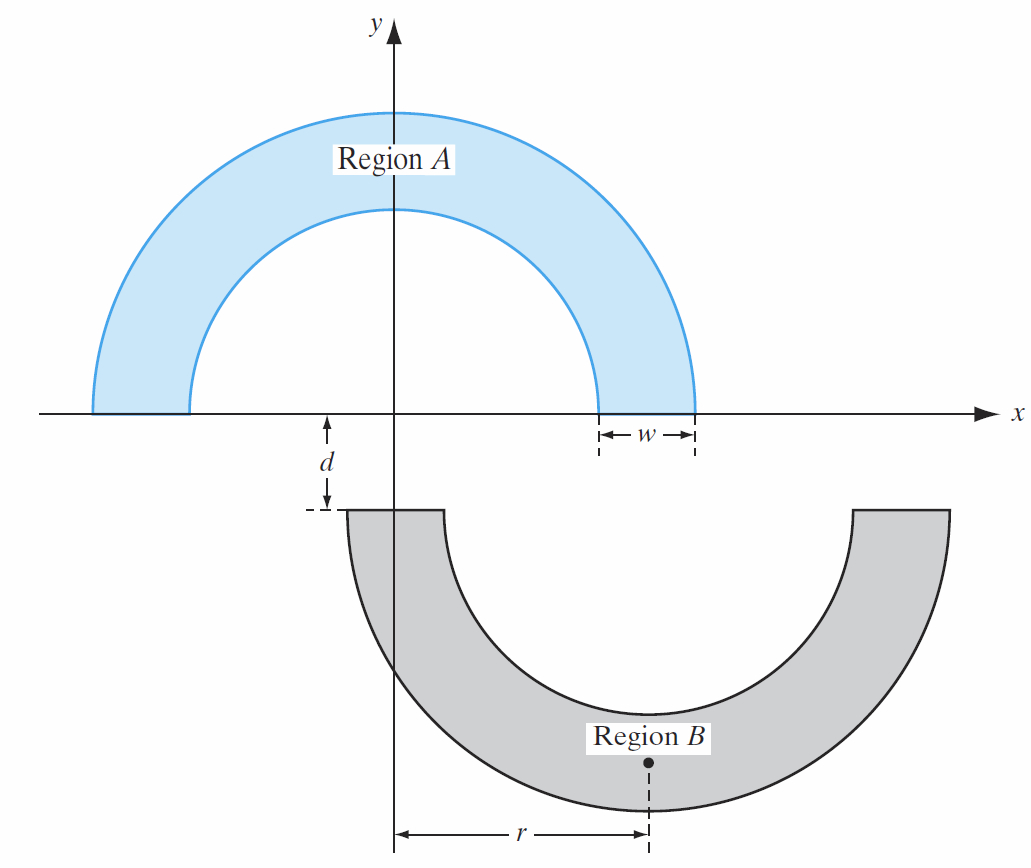
\includegraphics[width=.6\columnwidth]{images/105doublemoon2}
\caption[Double moon scheme]{Double moon scheme \cite{RefWorks:158}.}
\label{fig:105doublemoon2}
\end{figure}
The classical example of the double moon, see Fig. \ref{fig:105doublemoon2},
which clarifies the limits of the single perceptron approach, especially 
why a single neuron is not capable to handle a
nonlinear problem.
We drew two \textit{moons}, both with an inner radius $r$. 
Their minimum distance is $d$.
We could consider the two moons as composed by a finite number of
two-dimensional points.
If we use a portion of these points to train the $perceptron$, i.e. 
to teach the network which points belong to a region and which belong to the
other.
Goal of the $perceptron$ is to divide the two-dimensional
into two separate regions.
As long as $d$ is positive, the investigation space
can easily be linearly separated in two regions.
Once trained, the $perceptron$ can assign the remaining points 
to one moon or the other according to the training.

\section{Multilayer}
\label{sec:multilayer}

\begin{figure}[!h]
\centering
\includegraphics[width=.70\columnwidth]{images/063doublemoon}
\caption[Double moon classification problem 1]{Double moon classification
problem \cite{RefWorks:158}. Literature challenge to distinguish between linear
and non linear separation algorithms.}
\label{fig:063doublemoon}
\end{figure}



The handling of multiple outputs or, in our example, 
when $d$ becomes negative, see Fig. \ref{fig:063doublemoon}, makes linear
separation not possible, and a multineuron approach necessary. 
\begin{figure}[!htb]
\centering
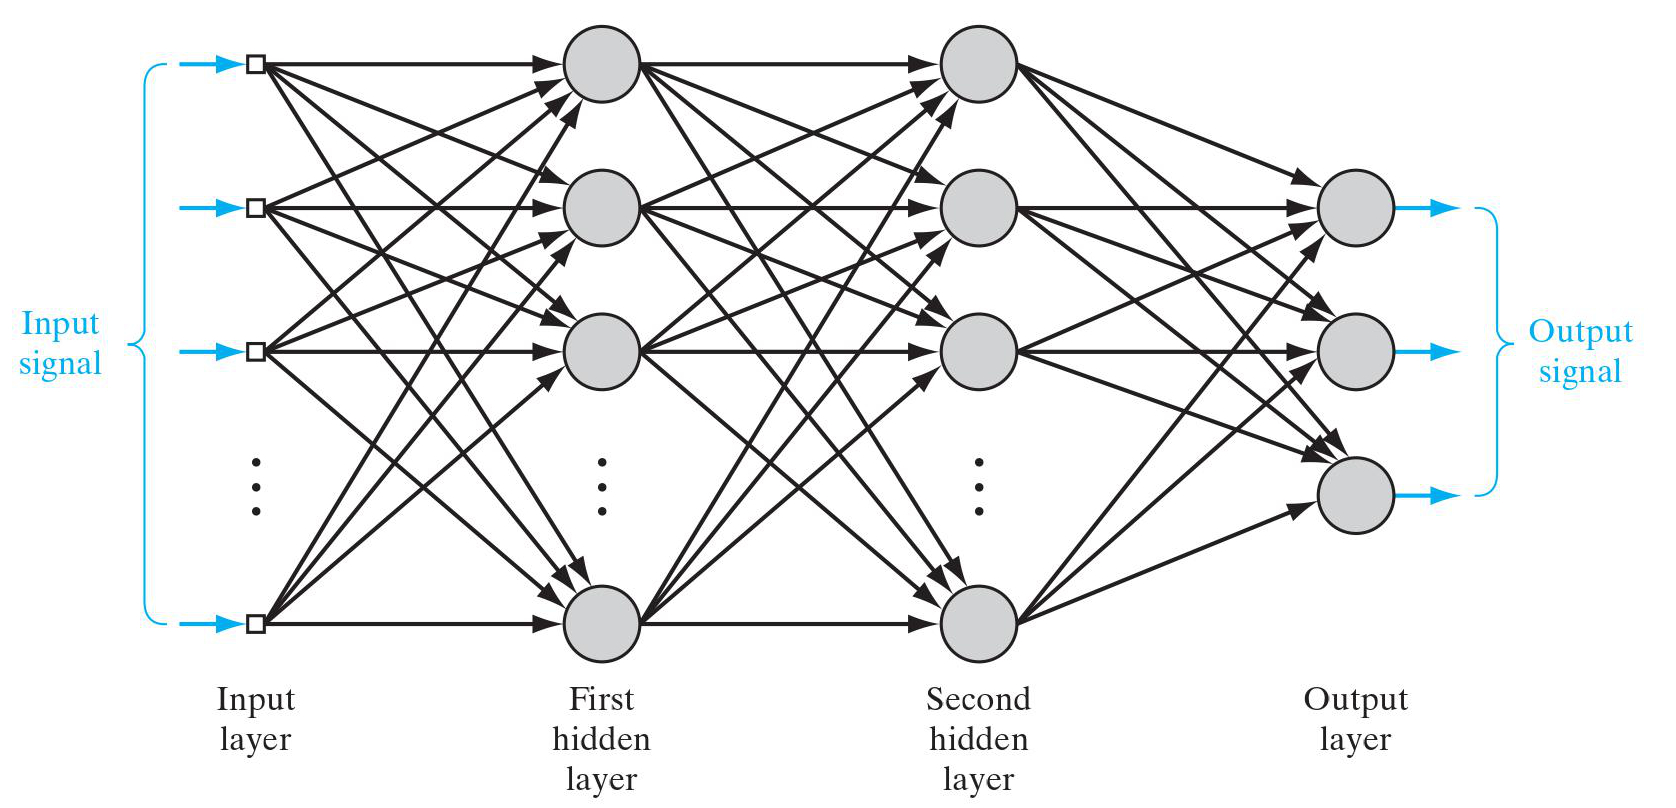
\includegraphics[width=.80\columnwidth]{images/111multilayerperceptron}
\caption[Multilayer perceptron]{Multilayer perceptron architecture, with
emphasys over the componing layers
\cite{RefWorks:158}.}
\label{fig:111multilayerperceptron}
\end{figure}
Many neurons are combined to form a network, as in the architecture presented
in Fig. \ref{fig:111multilayerperceptron}.
With more neurons, we can obtain a non-linear solution of our separation
problem, and correctly classify the input, as shown in Fig.
\ref{fig:063doublemoon}.\\
The first requirement of a multilayer neural network is that each neuron 
of the network must have differentiable nonlinear activation
function, such as the strictly increasing hyperbolic tangent.
Further, the network must have at least one layer $hidden$ from both the input
and the output nodes, see Fig. \ref{fig:018nnscheme}, to compute higher-order
statistics.\\
An high degree of $connectivity$ is another salient characteristic, dependent on
the synaptic weights of the network.
Usually, each neuron of one layer is linked with all the neurons in the previous
layer.
A network is called \acs{FF} if the inputs of the neurons in
one layer are exclusively the output signals of the neurons in the previous
layer.\\

%\improvement{Add some more details about the multilayer from Haykin}
%\improvement{explain feed forward here, pag 21 haykin}

\section{Batch Learning}
\label{sec:batchlearning}

A Multilayer \acs{ANN} can be trained in a supervised fashion with a training
sample
\begin{equation}
\label{eq:trainingsample}
\mathscr{T} = \{\mathbf{x}(n), \mathbf{d}(n) \}^N_{n = 1},
\end{equation}

where $\mathbf{x}(n)$ is the stimulus applied to the input layer.
The error is calculated 
as the difference at the j-th
node between the output of the neuron ($y_j(n)$) and the expected response
($d_j(n)$):
\begin{equation}
\label{eq:error}
e_j(n) = d_j(n) - y_j(n).
\end{equation}

$\mathbf{d}(n)$ is the desired response vector, and $d_j(n)$ is its j-th
element.
As in the Least Mean Square algorithm (see \citet{RefWorks:158}), we define
the \textit{instanteneous error energy} for the j-th neuron as:
\begin{equation}
\label{eq:insterrorenergy}
\mathscr{E}_j(n) = \frac{1}{2}
\mathit{e}_j^2(n).
\end{equation}

If we sum over all the neurons in the output layer, we obtain
the \textit{total instanteneous error energy} as:
\begin{equation}
\label{eq:totalinsterrorenergy}
\begin{align*}
\mathscr{E}(n) & = \sum_{j \in C}{\mathscr{E}_j(n)} \\
			   & = \frac{1}{2} \sum_{j \in C}{\mathit{e}_j^2(n)}
\end{align*}
\end{equation}

One $epoch$ of training consists in the calibration of the synaptic weights
after the presentation of all the $N$ training samples in $\mathscr{T}$
Thus,
% With a total of $N$ expected responses for training 
the cost function (\acs{EW}) to be minimized can be
expressed as the \textit{error energy averaged over the training sample}:
\begin{equation}
\label{eq:costfunction}
\mathscr{E}_{av}(N) = \frac{1}{N}
\sum_{n=1}^{N}{\mathscr{E}_n(N)}.
\end{equation}

In the following epoch, the training sample $\mathscr{T}$ is randomly shuffled,
and the cost function is once more computed.
We define the \textit{gradient vector}
\textbf{g}(\textit{n}) as:
\begin{equation}
\label{eq:gradientvector}
\mathbf{g}(\mathit{n}) = 
\left. \frac{\partial \mathscr{E}_{av}(\mathbf{w})}{\partial
\mathbf{w}}\right|_{\mathbf{w}=\mathbf{w}(\mathit{n})} ,
\end{equation}

or the derivative of the cost function over the  weight vector.
The \textit{batch learning} method grants an accurate prediction of the
\textit{gradient vector}, and consequently, given defined prerequisites, the
convergence to a local minimum of the method of the steepest descent.


\section{Backpropagation algorithm}
\label{sec:backpropagationalgorithm}

% If we consider a single perceptron, each example consists of a vector of inputs
% and a scalar expected response.
\citet {RefWorks:158} defines the induced local field for a multilayer
\acs{ANN} as:
\begin{equation}
v_j(n) = \sum_{i = 0}^{m}{w_ji(n) \cdot y_i(n)},
 \label{eq:inducedlocalfieldml}
\end{equation}

for the j-th neuron and the n-th example, given $m$ inputs.
The case of $i$ equal to zero refers to the bias.
Consequently, the function signal $y_j(n)$ for neuron $j$ becomes: 
\begin{equation}
y_j(n) = \varphi(v_j(n)).
 \label{eq:perceptronml}
\end{equation}

Thus, the weight $w_{ji}(n)$ of the $i$-th input for the $j$-th neuron
with the $n$-th example is corrected by the back-propagation algorithm as
follow:
\begin{equation}
\label{eq:deltaweight}
\Delta w_{ji}(n) = -\eta \frac{\partial \mathscr{E}(n)}{\partial
\mathit{w}_{ji}(n)},
\end{equation}

where the fraction represents the \textit{sensitivity factor} and \acs{eta} is
the \textit{learning-rate parameter}, which could be a user tuned parameter.
We can also write it as proportional to the \textit{local gradient}
$\delta_j(n)$:
\begin{equation}
\label{eq:deltaweight2}
\Delta w_{ji}(n) = -\eta \delta_j(n) y_i(n) .
\end{equation}

A multilayer perceptron network can be trained with the
supervised back-propagation algorithm, composed of two phases, forward and
backward, as shown in Fig. \ref{fig:112ffbp}.
\begin{figure}[!htb]
\centering
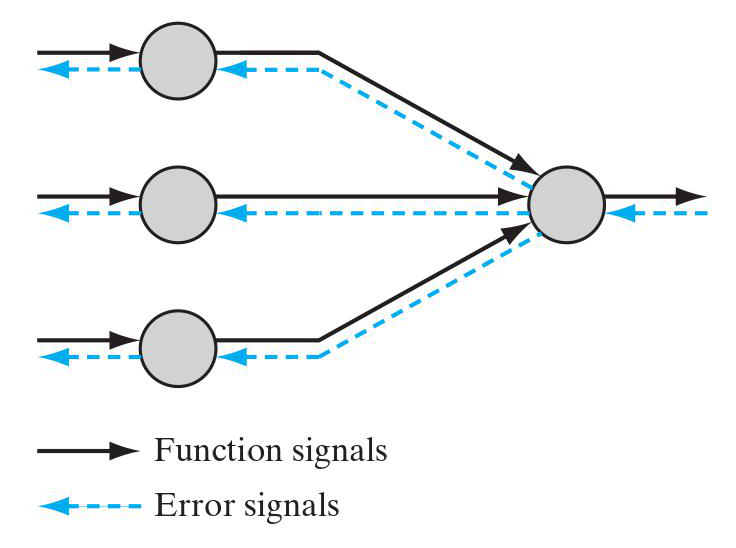
\includegraphics[width=.50\columnwidth]{images/112ffbp}
\caption[\acs{FF} Backpropagation]{\acs{FF} Backpropagation
\cite{RefWorks:158}.}
\label{fig:112ffbp}
\end{figure}
In the first phase the weights do not change. 
From the inputs through the hidden
and output layers the output is computed.
The backward pass moves in the opposite direction, from right to left.
The local gradient $\delta$ is computed for each neuron, layer by layer.
Thus, the weights can be tuned accordingly to the delta rule of Eq.
\ref{eq:deltaweight2}.\\
The variations of the weights in each loop can be more or less consistent,
accordingly to the learning-rate parameter \acs{eta}. 
A large \acs{eta} makes the algorithm fast,
while a small one prevents divergence.
Converged is reached when the absolute rate of change in the average squared
error per epoch is sufficiently small \cite {RefWorks:158}.
In our case, when $\mathscr{E}_{av}(N) < 10^{-4}$.\\
% In the second phase the error is calculated 
% and used to tune the weights, backward from the output to hidden
% layers.
% Of course, it arises the problem of when stopping the loop (or epoch). 
% Thus, a cost
% function  is defined: 
% in each loop of
% the algorithm its value is lower than in the previous loop.
% If we consider $C$ neurons in the output layer the 
% \textit{total instantaneous error energy} of the whole network is:
% \wrong{rephrase after missing paragraph}
% where 

% \subsection{Backpropagation computational steps}
% \label{subsec:backpropagationcomputationalsteps}
% 
% \citet {RefWorks:158} defines 

\subsection{Backpropagation efficacy}
\label{subsec:backpropagationefficacy}

The validity of the \textit{\acs{FF} Multilayer Perceptron Neural Networks}
(\acs{MLPNN}), with a backpropagation reinforcement learning training algorithm,
% (scaled conjugate gradient)
has been demonstrated in the 
literature, see \citet{RefWorks:158}. Several scientists 
\cite{RefWorks:161, RefWorks:166, RefWorks:167, RefWorks:168, RefWorks:169,
RefWorks:170, RefWorks:178, RefWorks:179} have employed \acs{ANNs} to model
the mechanical properties of materials.

\section{Optimization}
\label{sec:optimization}

Expanding this vision to multineurons network shifts into a matrix of inputs and
a vector of expected responses and consequently a vector of errors, from which
we can derive an error surface. 
\wrong{insert the equation system}
The quadratic approximation of the error surface can be performed with the
following methods:

\begin{itemize}
  \item{conjugate gradient,}
  \item{Newton and quasi-Newton,}
  \item{Levenberg-Marquardt.}
\end{itemize}

Compared to a linear approximation the conjugate gradient method is 
more precise. 
Further, it is faster and less computationally demanding than the
remaining quadratic methods.



First, the weights are randomly initialized. 
At every iteration the n-th example is used to computed $\eta$, and later
explicetely the weights $(n + 1)$'th iteration are obtained.
Then \textbf{g}(\textit{n + 1}) is calculated, to be later used with the
Polak-Ribiere method to compute the direction vector.
The gradient methods stops when the residuals, calculated from the
\acs{EAVN}, reach convergence.

% To be able to handle non-linearly separable data, the standard linear perceptron
% \acs{ANN} was modified to obtain \textit{FF Multilayer Perceptron Neural Networks
% (MLPNN)}.
% Here, each processing unit or node (neuron) possesses a nonlinear activation function. 
% They are interconnected to form layers that are also interlinked. 

\section{Generalization}
\label{sec:generalization}

\begin{figure}[htbp]
  %\null\hfill
  \subfloat[Good fitting.]{
	  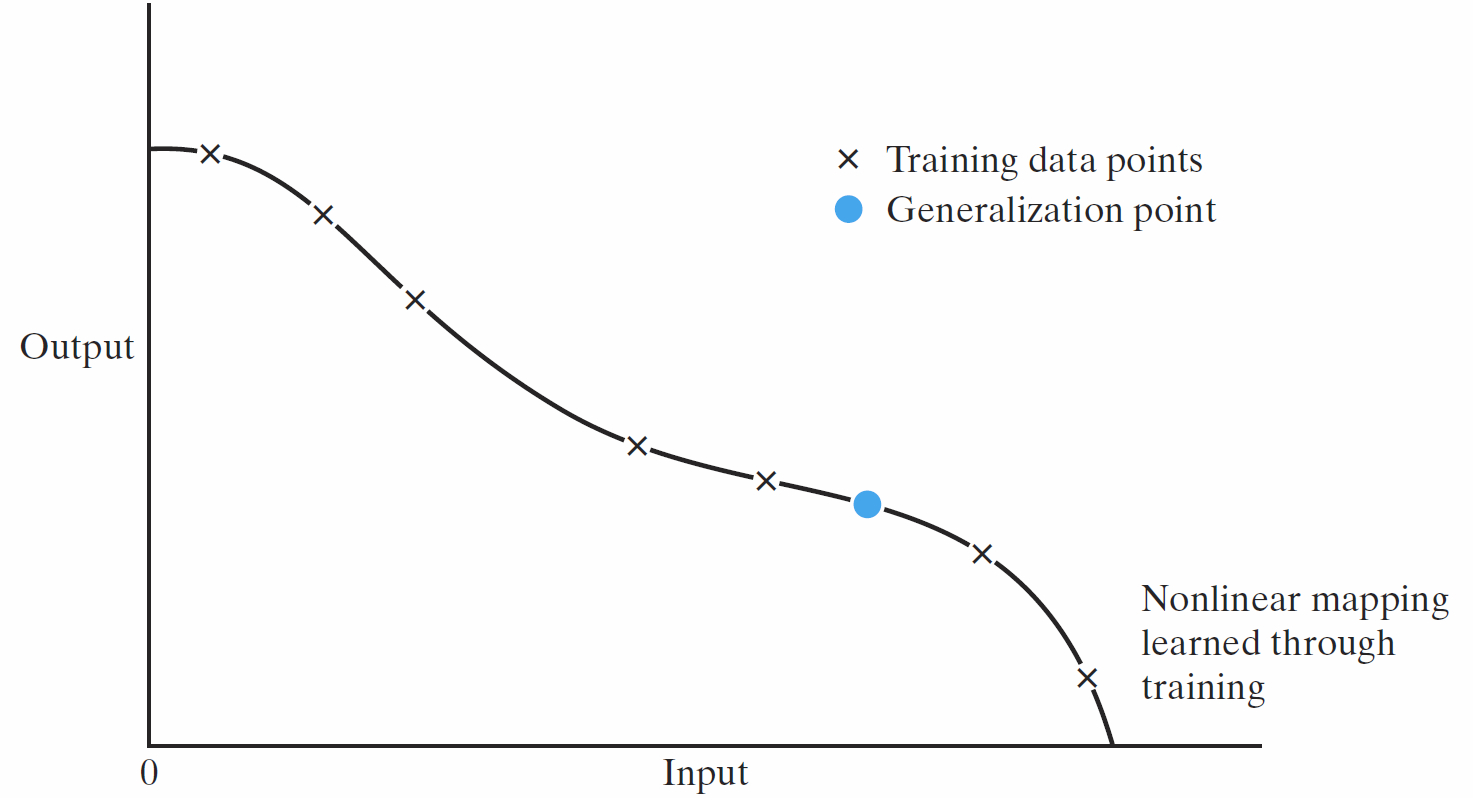
\includegraphics[width=.47\columnwidth]{images/106goodfitting}
	  \label{fig:106goodfitting}  }
  \quad
 % \hfill
  \subfloat[Bad fitting.]{
	  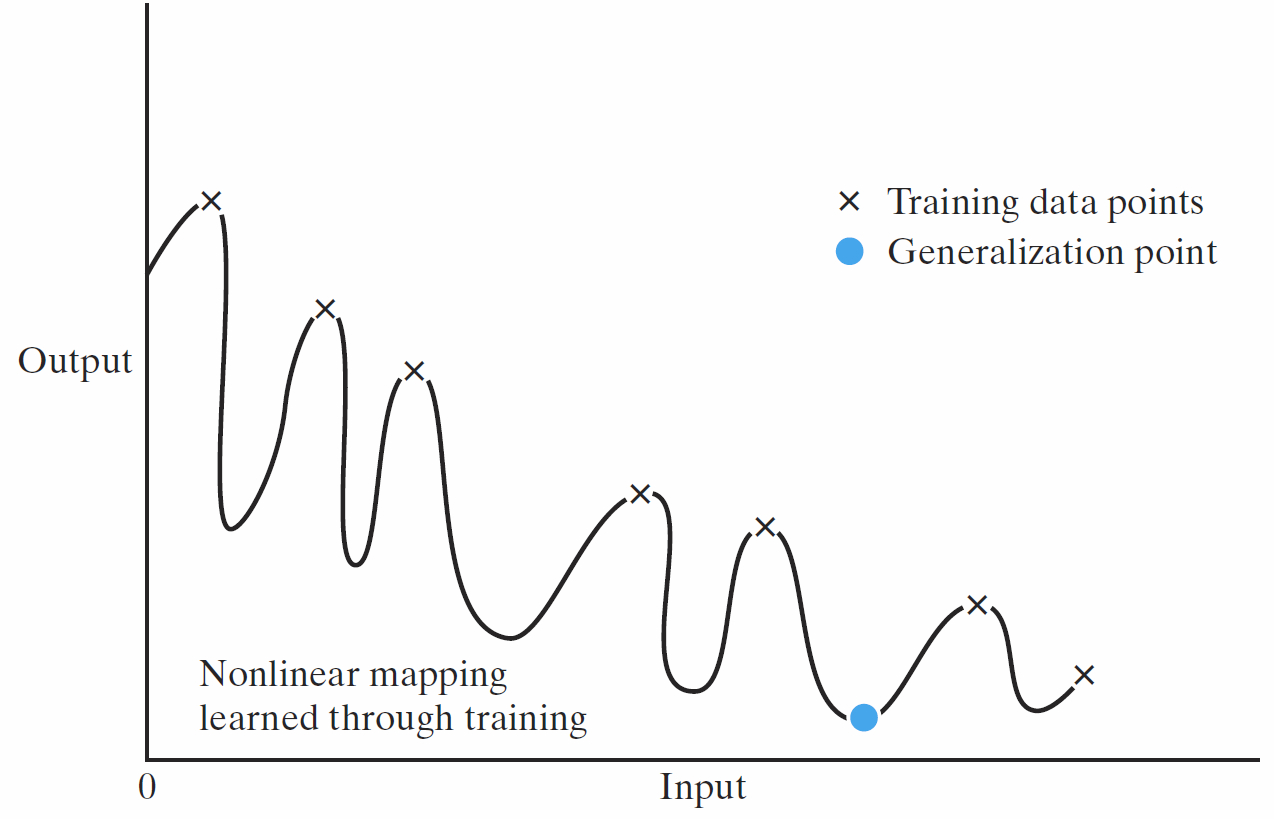
\includegraphics[width=.47\columnwidth]{images/107badfitting}
	  \label{fig:107badfitting}
  }
 % \hfill\null
  \caption[Fitting.]{Fitting, or agreement, between data point and
  regression, or interpolation, functions
  \cite{RefWorks:158}.}
  \label{fig:108fitting}
\end{figure}

\citet {RefWorks:158} suggests to carefully analyze two extreme situations:
\begin{itemize}
  \item {underfitting (or undertraining),}
  \item {overfitting (or overtraining),}
\end{itemize}
when training a network.\\
Correctly computed input-output mapping is a synonym of a well $generalized$
network, and of good nonlinear interpolation of the inputs, as in Fig. 
\ref{fig:106goodfitting}. 
On one hand, $underfitting$ means that there were not neurons to characterize
the given function.\\
On the other hand, an excessive amount of
training samples, known as $overfitting$, leads to poor generalization, see 
Fig. \ref{fig:107badfitting}. Also the architecture of the neural network and
physical complexity of the problem influence the generalization.
A good rule of thumb requires the size of the training sample to be of the same
order of magnitude of the ratio between:
\begin{enumerate}[label=(\alph*)]
  \item{the total number of free parameters (i.e., synaptic weights and biases)
  in the network,}
  \item{the fraction of classification errors permitted on test data (e.g., the
  mean square value of the estimation error).}
\end{enumerate}

\section{Cross validation}
\label{sec:crossvalidation}

A computationally efficient training and the evaluation of good generalization
can be performed with the statistical tool of \textit{cross-validation}.
The available data are randomly divided in the following subsets:

\begin{enumerate}
  \item{training samples subset,}
  \item{generalization (or validation, or early stopping) samples subset,}
  \item{test samples subset.}
\end{enumerate}

For instance, every ten epochs the training is halted and the validation error
(or the cost function) is evaluated with the partially trained network over the
validation set.
Then the training is resumed. \\
This continues until the learning curve of the error for the validation set
reaches a local minimum, a condition that should happen sooner (i.e., in a
minor number of loops) than the falling of the learning curve for the training
set (cost function \acs{EAVN}) under the prescribed limit.
At this point the output of the trained network is evaluated over the test
subset to evaluate its generalization performances.\\
Also the standard regression models (i.e., Bayesian and Gaussian) are similarly
evaluated.

\section{ANNs training for DEM identification}
\label{sec:annstrainingfordemidentification}

In their work, \citet{RefWorks:150} suggest an effective algorithm for
\acs{MLPNN} regression. We followed their instructions. \\
Further, the quality of the \acs{ANN} data had to be examined critically. 
\citet{RefWorks:158} 
suggested considering the quality of:
\begin{enumerate}[label=(\alph*)]
  \item {\acs{ANN} training process,}
  \item {the subsequent data generation based on the inputs provided.}
\end{enumerate}

Task (a) is particularly important
when dealing with experimental training data, and
usually addressed
by noise-corrupted pattern calibration
and by comparison with standard statistical methods.
However, our training pool was numerical and extensive, 
and the particles in our simulations were inserted using a random
seed value.
For vast amounts of training data, the effect of noise-corrupted patterns is
negligible, see \citet{RefWorks:158}. \\
Thus, in our work task (b) was more challenging.
Once trained, the \acs{ANN} were fed
combinations of \acs{DEM} parameters. 
We tried different methods to generate these combinations. 
Our first attempt consisted of assigning parameters to the investigated
variables in even increments from the minimum to the maximum values. 
For example, the \acs{CoR} ranged from 0.5 to 0.9, and thus the first value was
0.5, the second 0.508163, and so on. \\
To increase generalization, we decided to follow a different approach: 
random value generators created the number of required values in the defined
ranges for each parameter investigated.
These were combined and used as input.\\

\section{Comparison of regression methods}
\label{sec:comparisonofregressionmethods}


\begin{table}[htbp]
  \centering

    \begin{tabular}{l|ccc}
    \hline
          & Bayesian & Gaussian & ANN \\
          \hline
    Cost function & maximum  & maximum & scaled \\
     			  & likelihood & likelihood & conjugated \\
     			  & estimation & estimation & gradient \\
    \hline
    \end{tabular}%
      \caption{Regression methods comparison.}
  \label{tab:17regressionmethods}%
\end{table}%